\documentclass{article}
\usepackage{pdfpages}
\usepackage{minted}
\usepackage[utf8]{inputenc}
\usepackage[spanish]{babel}
\usepackage{csquotes}
\MakeOuterQuote{"}
\usepackage{caption}
\usepackage{enumitem}
\usepackage{graphicx}
\definecolor{bg}{rgb}{0.95,0.95,0.95}

\begin{document}

\tableofcontents

\newpage

\section{Crear un proyecto Java para BPMN 2.0}
\subsection{Crear un nuevo proyecto Maven en Eclipse}

En Eclipse, anda a: File / New / Other .... esto abre el asistente de nuevo proyecto. En el asistente, selecciona: Maven / Maven Project. Clicka "Next".

\begin{center}
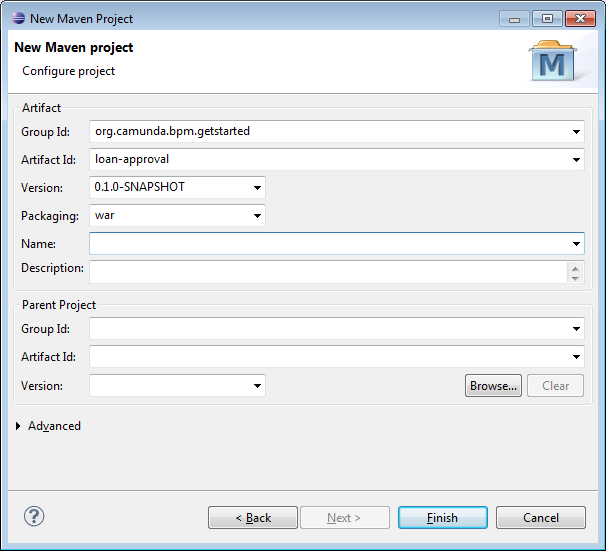
\includegraphics[width=\textwidth, height=10cm]{eclipse-new-project.png}
\end{center}

En la primera página del asistente, selecciona "Create a simple proyect" (Ignora "archetype selection"). Clicka "Next".

En la segunda página (ver imagen), configura los atributos del proyecto Maven. Como estamos configurando un proyecto "war", asegúrate de seleccionar "Packaging: war".

Cuando estés listo, clicka "Finish". Eclipse creará un nuevo proyecto Maven. El proyecto aparecerá en "Project Explorer View".


\newpage
\subsection{Agregar dependencias Camunda Maven}

El siguiente paso consiste en configurar las dependencias Maven para la nueva aplicación. Agrega las siguientes dependecias al archivo pom.xml del proyecto:

\begin{minted}[bgcolor=bg]{xml}
<project xmlns="http://maven.apache.org/POM/4.0.0" 
xmlns:xsi="http://www.w3.org/2001/XMLSchema-instance"
xsi:schemaLocation="http://maven.apache.org/POM/4.0.0 
http://maven.apache.org/xsd/maven-4.0.0.xsd">
  <modelVersion>4.0.0</modelVersion>
  <groupId>org.camunda.bpm.getstarted</groupId>
  <artifactId>loan-approval</artifactId>
  <version>0.1.0-SNAPSHOT</version>
  <packaging>war</packaging>

  <dependencyManagement>
    <dependencies>
      <dependency>
        <groupId>org.camunda.bpm</groupId>
        <artifactId>camunda-bom</artifactId>
        <version>7.8.0</version>
        <scope>import</scope>
        <type>pom</type>
      </dependency>
    </dependencies>
  </dependencyManagement>

  <dependencies>
    <dependency>
      <groupId>org.camunda.bpm</groupId>
      <artifactId>camunda-engine</artifactId>
      <scope>provided</scope>
    </dependency>

    <dependency>
      <groupId>javax.servlet</groupId>
      <artifactId>javax.servlet-api</artifactId>
      <version>3.0.1</version>
      <scope>provided</scope>
    </dependency>
  </dependencies>

  <build>
    <plugins>
      <plugin>
        <groupId>org.apache.maven.plugins</groupId>
        <artifactId>maven-war-plugin</artifactId>
        <version>2.3</version>
        <configuration>
          <failOnMissingWebXml>false</failOnMissingWebXml>
        </configuration>
      </plugin>
    </plugins>
  </build>

</project>
\end{minted}

Ahora, puedes ejecutar la primera compilación. Haz click derecho sobre pom.xml en el explorador de paquetes y selecciona "Run as / Maven Install".


%Falta Agregar las dependencias de esto%%%%%%%%%%%%%
\subsection{Agregar un "Process Application Class"}%
%%%%%%%%%%%%%%%%%%%%%%%%%%%%%%%%%%%%%%%%%%%%%%%%%%%%

Ahora, necesitas crear un paquete, por ejemplo:\\
org.camunda.bpm.getstarted.loanapproval. Agrega un "Process Application Class" en el paquete. "Process Application Class" constituye la interfaz entre tu aplicación y el motor de proceso.

\begin{minted}[bgcolor=bg]{Java}
package org.camunda.bpm.getstarted.loanapproval;

import org.camunda.bpm.application.ProcessApplication;
import org.camunda.bpm.application.impl.ServletProcessApplication;

@ProcessApplication("Loan Approval App")
public class LoanApprovalApplication extends ServletProcessApplication {
  // empty implementation
}
\end{minted}

\newpage
\subsection{Agregar un descriptor de despliegue \\"META-INF/processes.xml"}

El último paso para terminar de configurar la aplicación es agregar el archivo del descriptor de despliegue "META-INF/processes.xml". Este archivo nos brinda una configuración declarativa de despliegue, actuando como motor del proceso.

Este archivo debe ser agregado en la carpeta "src/main/resources/META-INF" del proyecto Maven.

\begin{minted}[bgcolor=bg]{xml}
<?xml version="1.0" encoding="UTF-8" ?>

<process-application
    xmlns="http://www.camunda.org/schema/1.0/ProcessApplication"
    xmlns:xsi="http://www.w3.org/2001/XMLSchema-instance">

  <process-archive name="loan-approval">
    <process-engine>default</process-engine>
    <properties>
      <property name="isDeleteUponUndeploy">false</property>
      <property name="isScanForProcessDefinitions">true</property>
    </properties>
  </process-archive>

</process-application>
\end{minted}

En este punto, tienes configurada satisfactoriamente tu aplicación y ya puedes empezar a modelar el primer proceso.

\newpage

\section{Modelando un proceso BPMN 2.0}

En esta sección, aprenderás cómo crear tu primer rpoceso BPMN 2.0 con Camunda Modeler. Ahora, inicia Camunda Modeler.

\subsection{Crea un nuevo diagrama BPMN 2.0}

Crea un nuevo diagrama BPMN clickando "File / New File / BPMN diagram"

\begin{center}
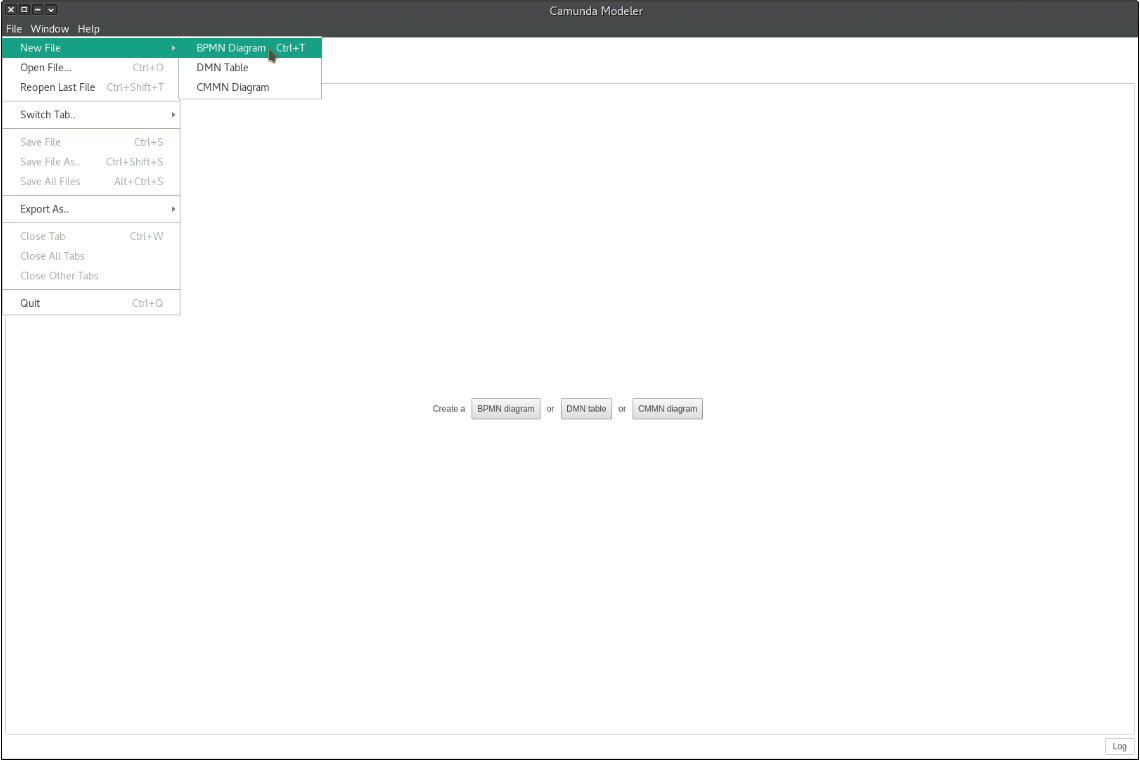
\includegraphics[width=\textwidth]{modeler-new-bpmn-diagram.png}
\end{center}

\subsection{Empieza con un proceso simple}
Empieza modelando un proceso simple.

\begin{center}
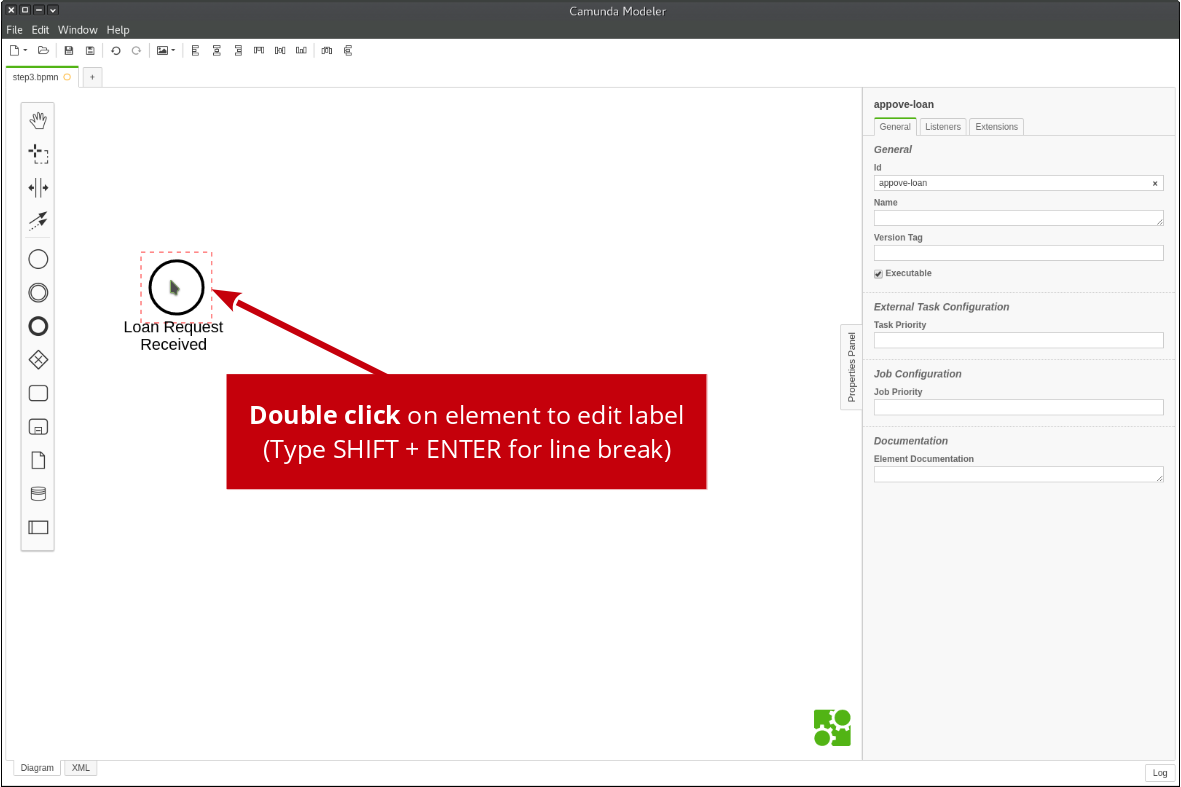
\includegraphics[width=\textwidth]{modeler-step1.png}
\end{center}

Haz doble-click sobre "Start Event". Una caja de texto se abrirá. Escribe “Loan Request Received”. Ahora, haz un click sobre "Start Event". Sobre el menú que se despliega, selecciona el rectángulo y desplázalo hacia una buena posición. Nómbralo "Approve Loan". Cambia el tipo de la actividad a "User Task", clickando sobre el rectángulo y luego clickando la llave inglesa.

\begin{center}
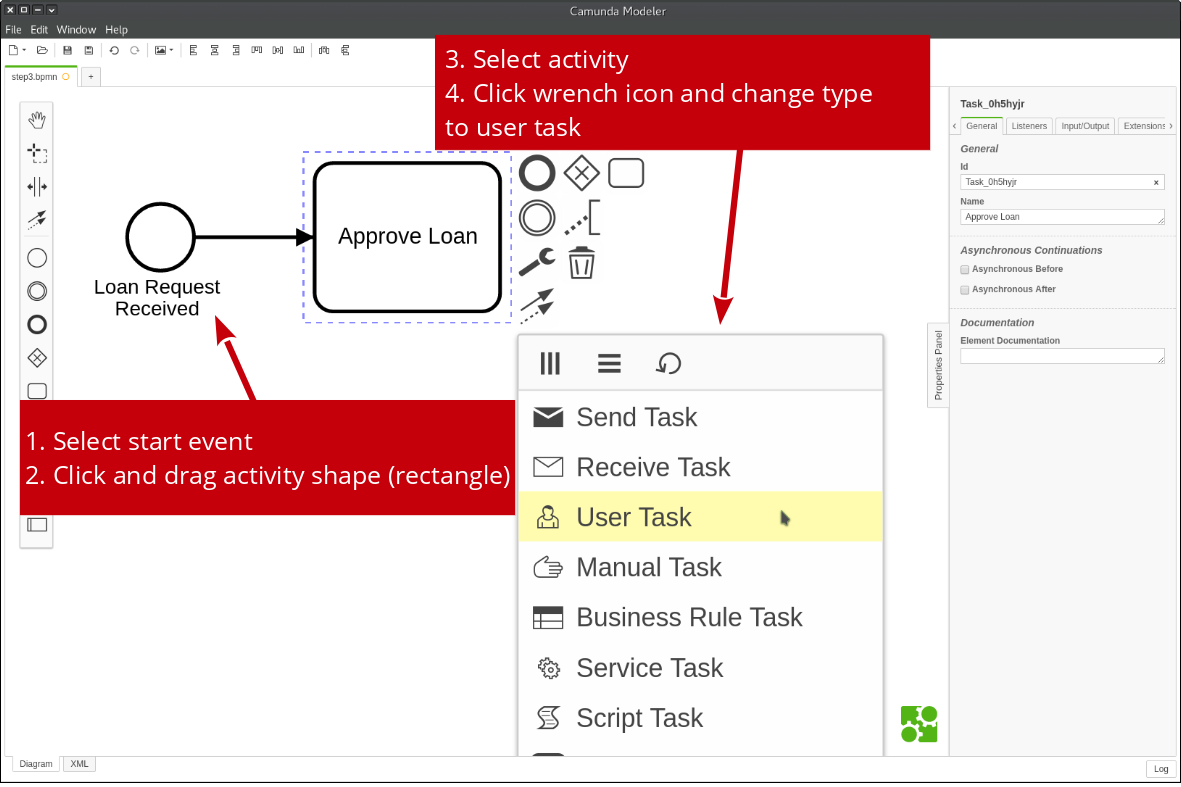
\includegraphics[width=\textwidth]{modeler-step2.png}
\end{center}

Clicka sobre el rectángulo que creaste, selecciona "End Event" y desplázalo a un posición adecuada. Nómbralo "Loan Request Approved".

\begin{center}
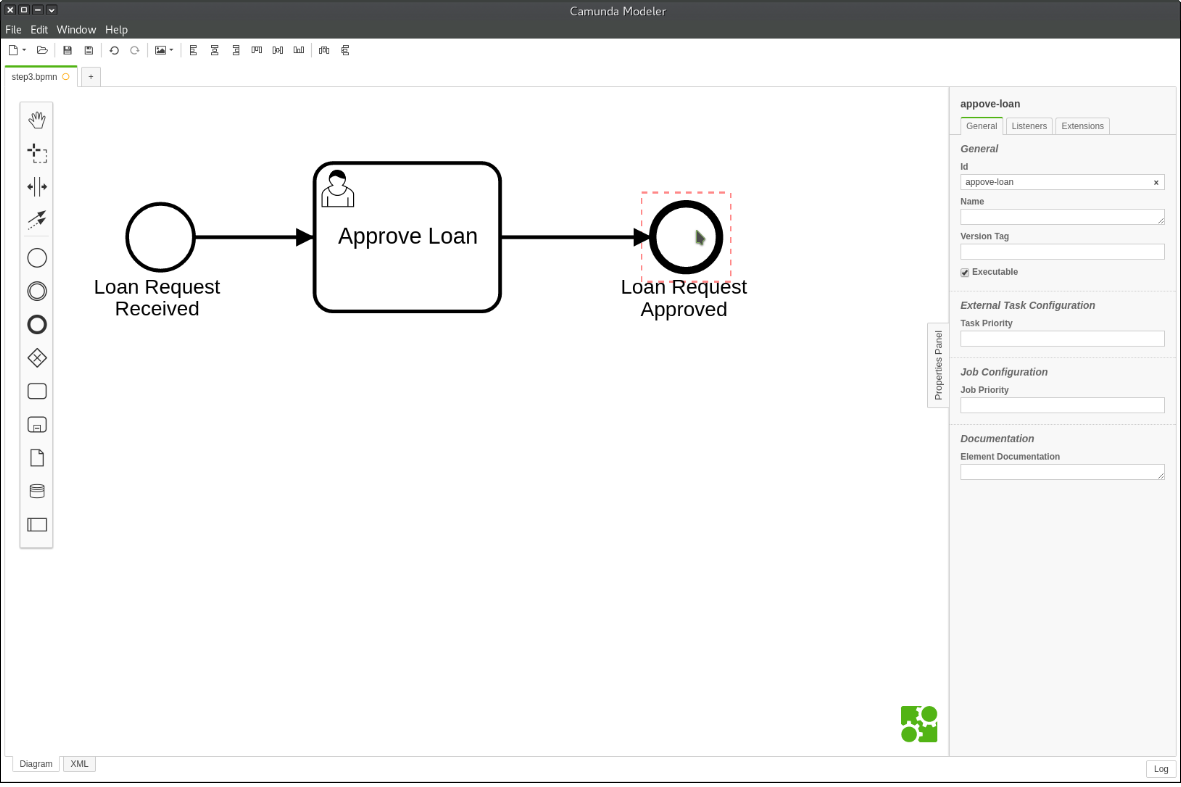
\includegraphics[width=\textwidth]{modeler-step3.png}
\end{center}

\subsection{Configura el "User Task"}

\begin{center}
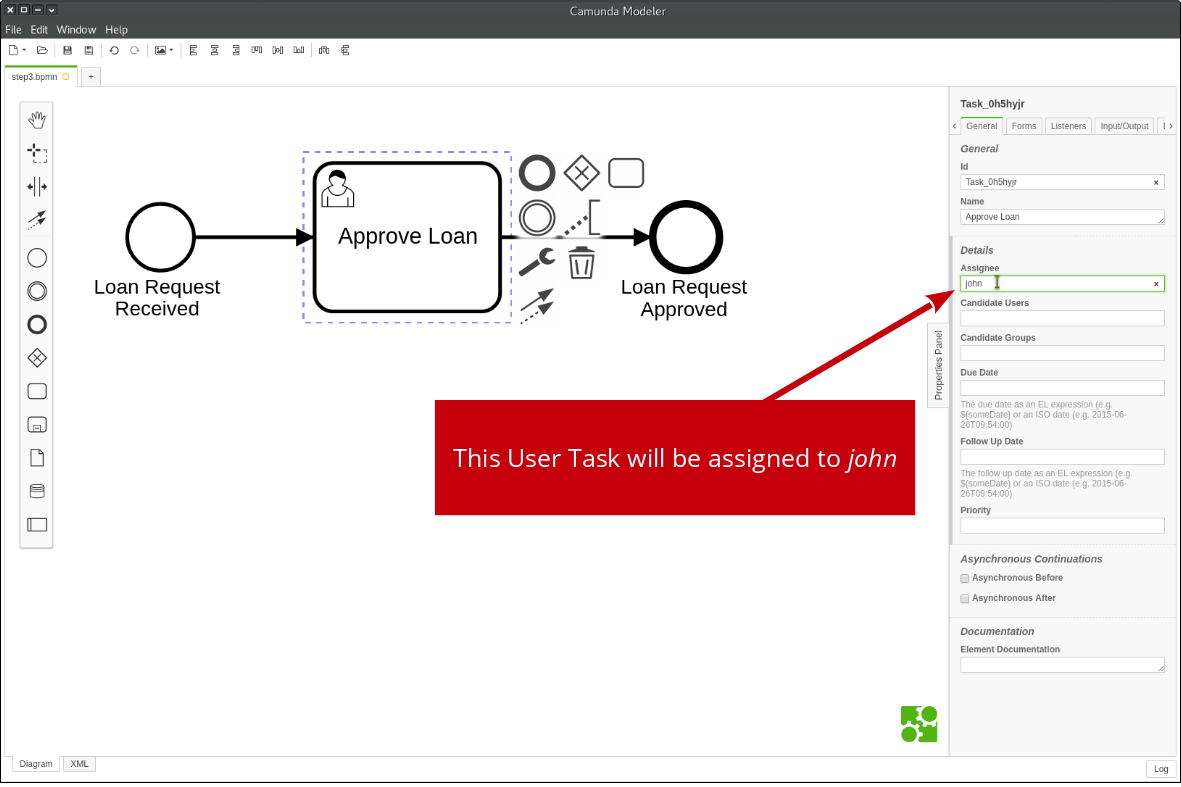
\includegraphics[width=\textwidth]{modeler-step4.png}
\end{center}

Ahora, abre la vista de propiedades. Si no está visible, clicka sobre la viñeta en la derecha de tu pantalla y la vista se desplegará.
Clicka sobre el "User Task". Esto actualizará la selección en la vista de propiedades. Baja hasta el campo llamado "Assignee" y escribe "john".
Cuando estés listo, guarda los cambios.

\subsection{Configura las propiedades para la ejecución}

\begin{center}
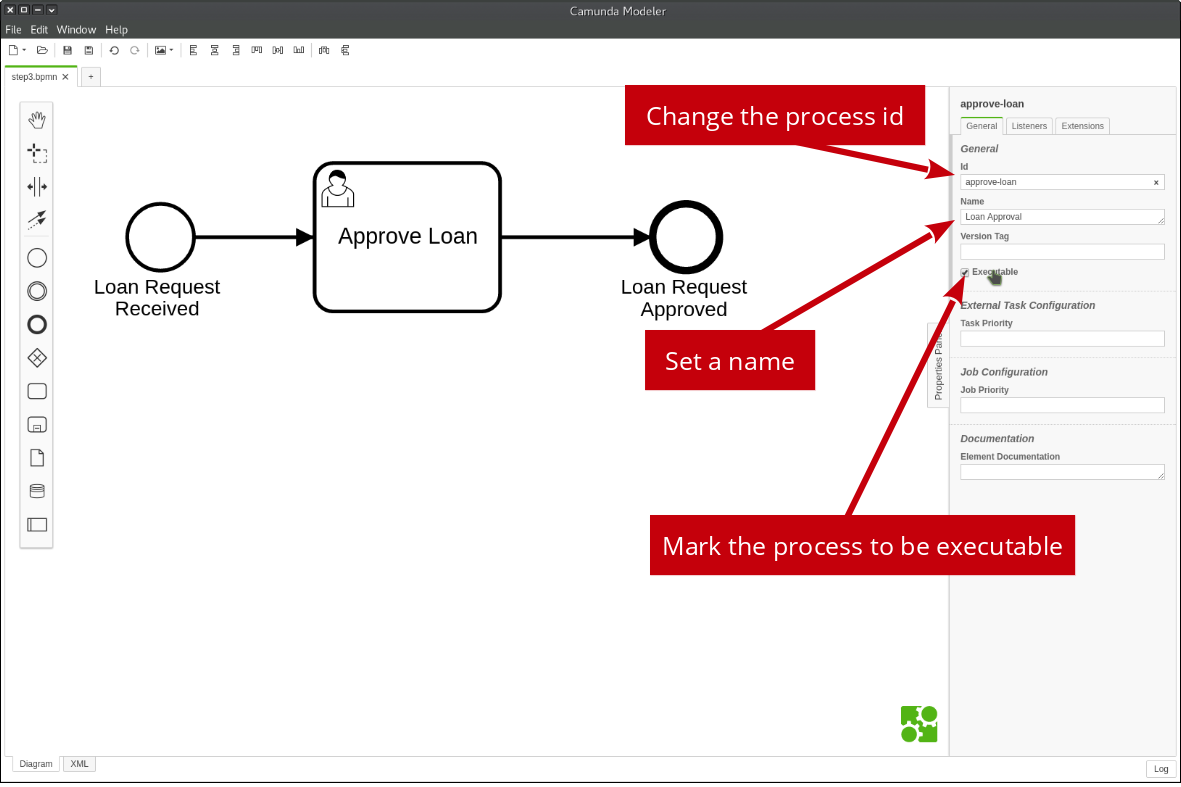
\includegraphics[width=\textwidth]{modeler-step5.png}
\end{center}

Como estamos modelando un proceso ejecutable, deberíamos darle un ID y configurar la propiedad "isExecutable" igual a "true". Clicka en un espacio vacío del diagrama para que se muestren las propiedades generales del flujo en la vista de propiedades.\\
Primero, configura un ID para el proceso. Escribe "approve-loan" en el atributo Id. El ID es usado por el motor del proceso como un identificador, y se considera una buena práctica darle un valor en lenguaje natural.\\
Segundo, configura el nombre del proceso. Escribe "Loan Approval" en el campo "Name".\\
Finalmente, clicka sobre el cuadro a la izquierda del atributo "Executable". Si no clickas este cuadro, la definción del proceso será ignorada por el motor de proceso.

\subsection{Guarda el diagrama BPMN}

\begin{center}
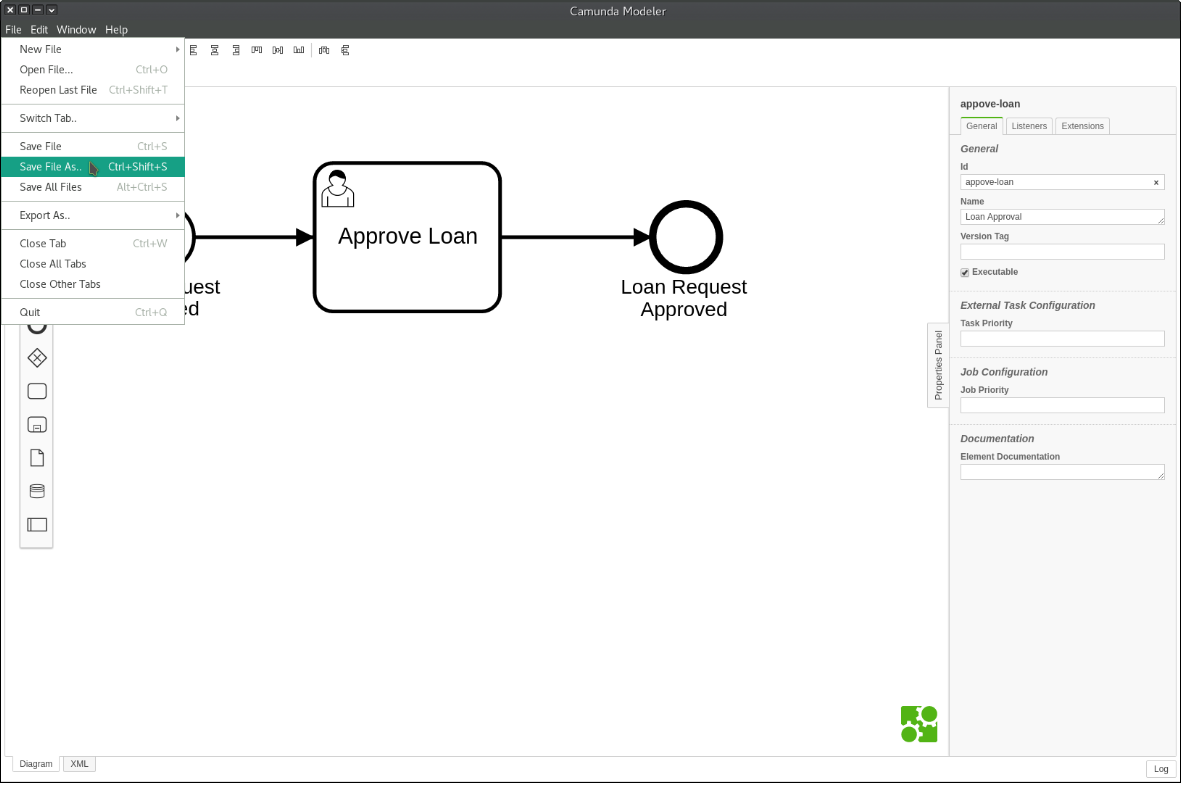
\includegraphics[width=\textwidth]{modeler-save-diagram.png}
\end{center}

Cuando estés listo, guarda tus cambios clickando "File / Save File As...". En la ventana que se desplegará, navega hacia donde tienes almacenado tu projecto Eclipse. En ese directorio, avanza hasta la carpeta "src/main/resources" y guarda ahí tu diagrama.\\
Vuelve a Eclipse. Haz click derecho sobre la carpeta del proyecto y clicka "Refresh". Esto sincronizará tu diagrama BPMN con Eclipse.

\newpage
\section{Despliega y testea el proceso BPMN 2.0}

El próximo paso consiste en compilar, desplegar y testear el proceso.

\subsection{Compila la aplicación web con Maven}

Slecciona pom.xml en el explorador de paquete, haz click derecho y selecciona "Runs As / Maven Install". Esto generará un archivo llamado "loan-approval-0.1.0-SNAPSHOT.war" en la carpeta "target" de tu proyecto Maven.
Si guardaste tu archivo BPMN del capítulo previo en "src/main/resources", entonces, el war que acabas de generar también lo incluye.

\subsection{Despliegue de Apache Tomcat}

Para desplegar la aplicación, copia y pega el archivo "loan-approval-0.1.0-SNAPSHOT.war" desde tu proyecto Maven a la carpeta "\$CAMUNDA\_HOME/server/apache-tomcat/webapps", donde "\$CAMUNDA\_HOME" es la ruta hacia tu servidor Camunda.
Revisa en el archivo log del servidor Apache Tomcat en la carpeta "\$CAMUNDA\_HOME/server/apache-tomcat/logs". Elige el archivo "catalina.out". Navega hasta el fin del archivo y, si ves el siguiente mensaje, el despliegue fue correcto:\\
\\

INFO org.camunda.commons.logging.BaseLogger.logInfo
ENGINE-07015 Detected @ProcessApplication class 'org.camunda.bpm.getstarted.loanapproval.LoanApprovalApplication'
INFO org.camunda.commons.logging.BaseLogger.logInfo
ENGINE-08024 Found processes.xml file at ../webapps/loan-approval-0.1.0-SNAPSHOT/WEB-INF/classes/META-INF/processes.xml
INFO org.camunda.commons.logging.BaseLogger.logInfo
ENGINE-08023 Deployment summary for process archive 'loan-approval':

        loan-approval.bpmn

INFO org.camunda.commons.logging.BaseLogger.logInfo
ENGINE-08050 Process application Loan Approval App successfully deployed

\subsection{Verifica el despliegue con Cockpit}

Ahora, usa Cockpit para verificar si el proceso fue desplegado satisfactoriamente. Anda a "http://localhost:8080/camunda/app/cockpit". Inicia sesión con "demo / demo". Tu proceso "Loan Approval" debiera ser visible en el "dashboard".

\begin{center}
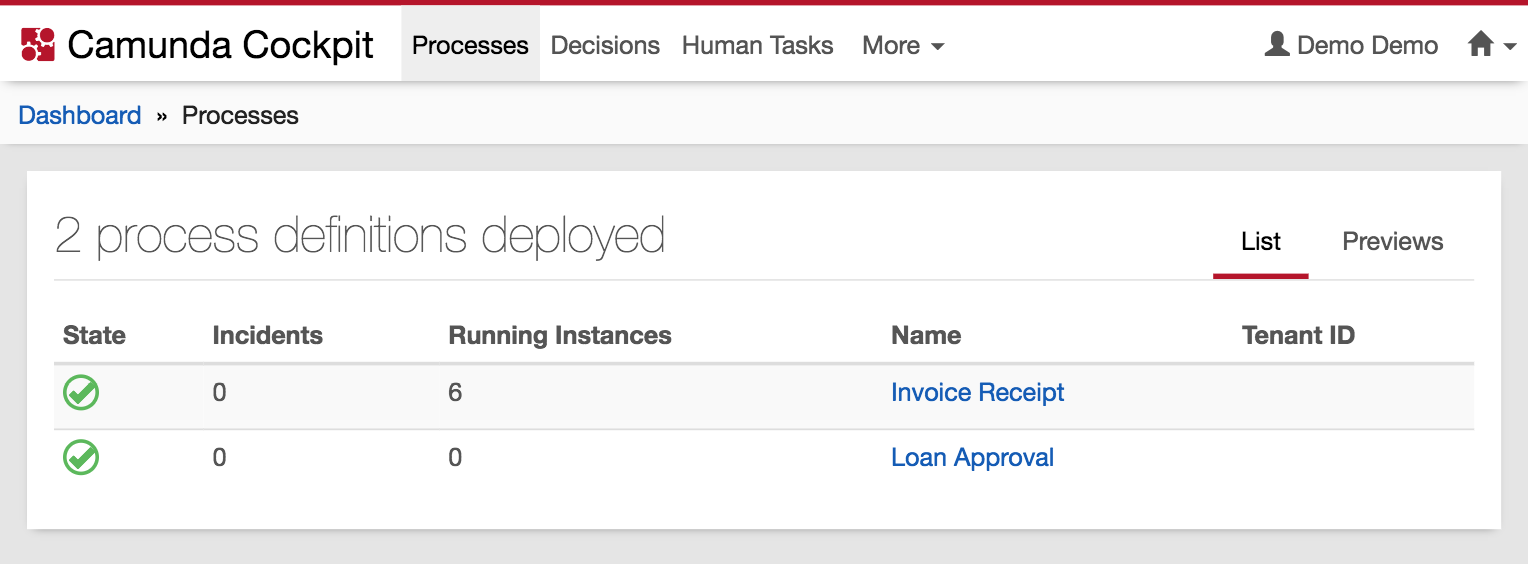
\includegraphics[width=\textwidth]{cockpit-loan-approval.png}
\end{center}

\subsection{Comienza una instancia del proceso}

Ahora, anda a "Tasklist" (http://localhost:8080/camunda/app/tasklist). Clicka en el botón "Start Process" para iniciar una instancia del proceso. Esto abre una ventana donde puedes seleccionar Loan Approval en la lista. Ahora, puedes configurar las variables para la instancia del proceso, usando un formulario genérico.

\begin{center}
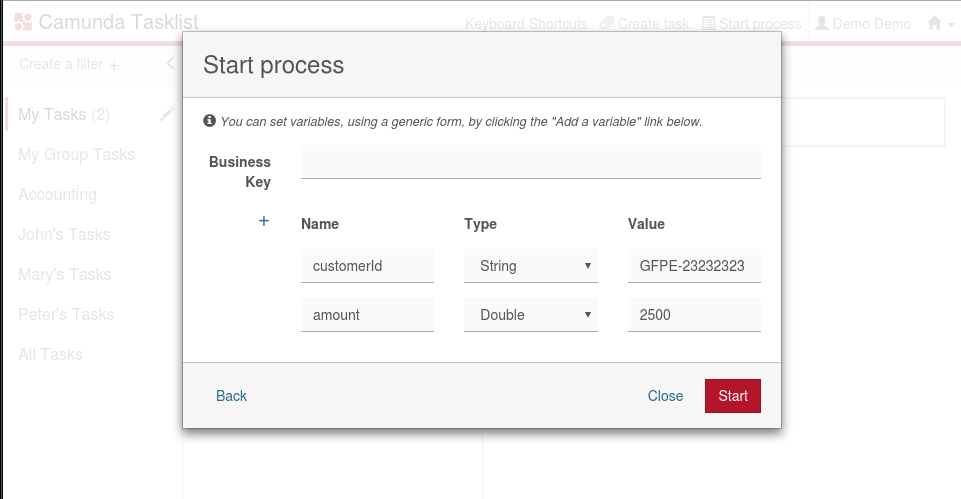
\includegraphics[width=\textwidth]{start-form-generic.png}
\end{center}

El formulario genérico se puede usar cuando no se ha agregado un formulario dedicado para un User Task o un Start Event. Clicka en el botón "Add Variable" para tener una nueva fila. Rellena el formulario como se muestra en la foto. Cuando estés listo, clicka "Start".
Si vuelves a Camunda Cockpit, verás creada una instancia nueva del proceso, la que está esperando en el "User Task".

\subsection{Configura las autorizaciones}

Para permitir al usuario john ver la definición del proceso Loan Approval, tienes que ir al Admin de Camunda (http://localhost:8080/camunda/app/admin/default/\#/authorization?resource=6). Luego, clicka en el botón "Create new authorization" para agregar una nueva autorización. Ahora, puedes darle al usuario john todos los permisos sobre la definición del proceso approve-loan. Cuando estés listo, agrega la nueva autorización.

\begin{center}
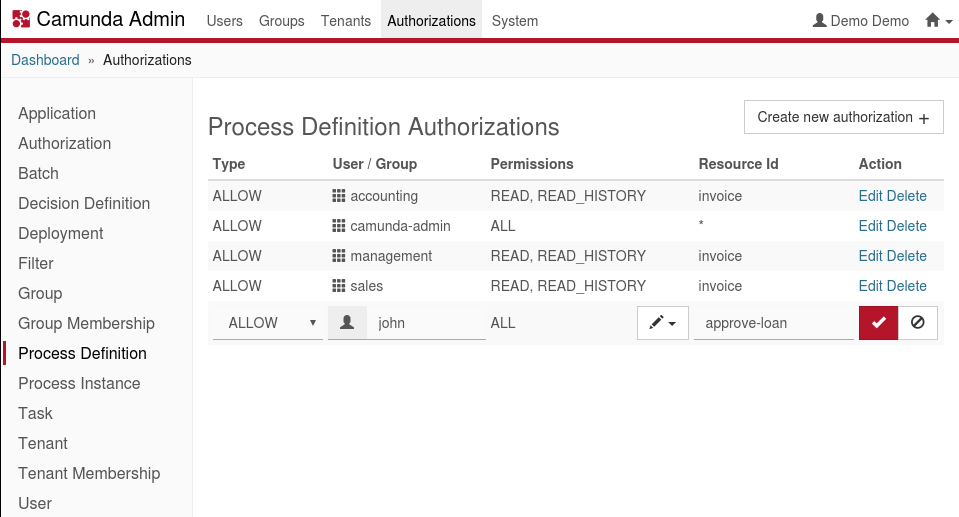
\includegraphics[width=\textwidth]{create-process-definition-authorization.png}
\end{center}

Ahora, crea una segunda autorización para la instancia del proceso. Configura el permiso a "CREATE".

\begin{center}
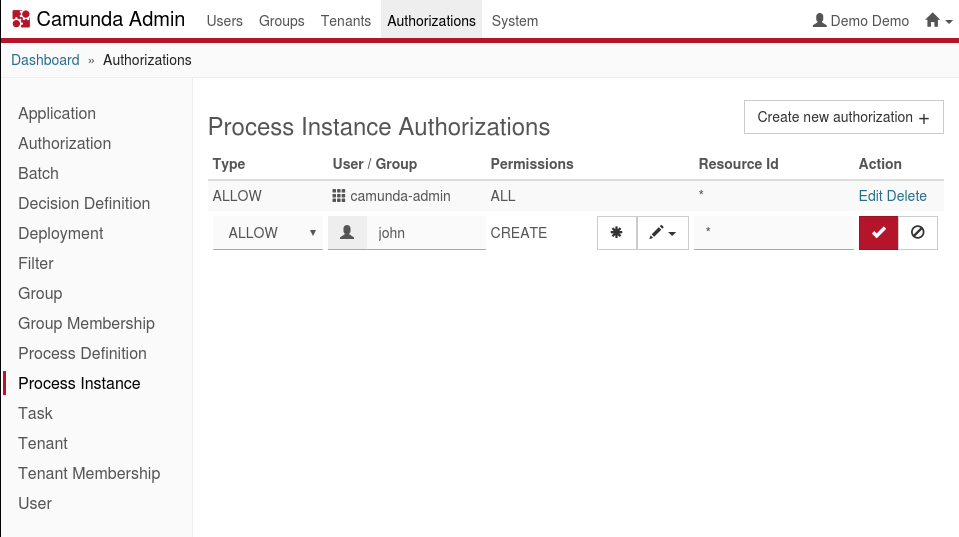
\includegraphics[width=\textwidth]{create-process-instance-authorization.png}
\end{center}

\subsection{Trabaja en el Task}

Cierra sesión de Admin. Anda al Tasklist (http://localhost:8080/camunda/app/tasklist) e inicia sesión con los datos "john / john". Ahora, verás el task Approve Loan en tu Tasklist. Selecciona el task y clicka en el tab "Diagram". Esto muestra el diagrama del proceso y remarca la tarea que está esperando a que trabajes en ella.

\begin{center}
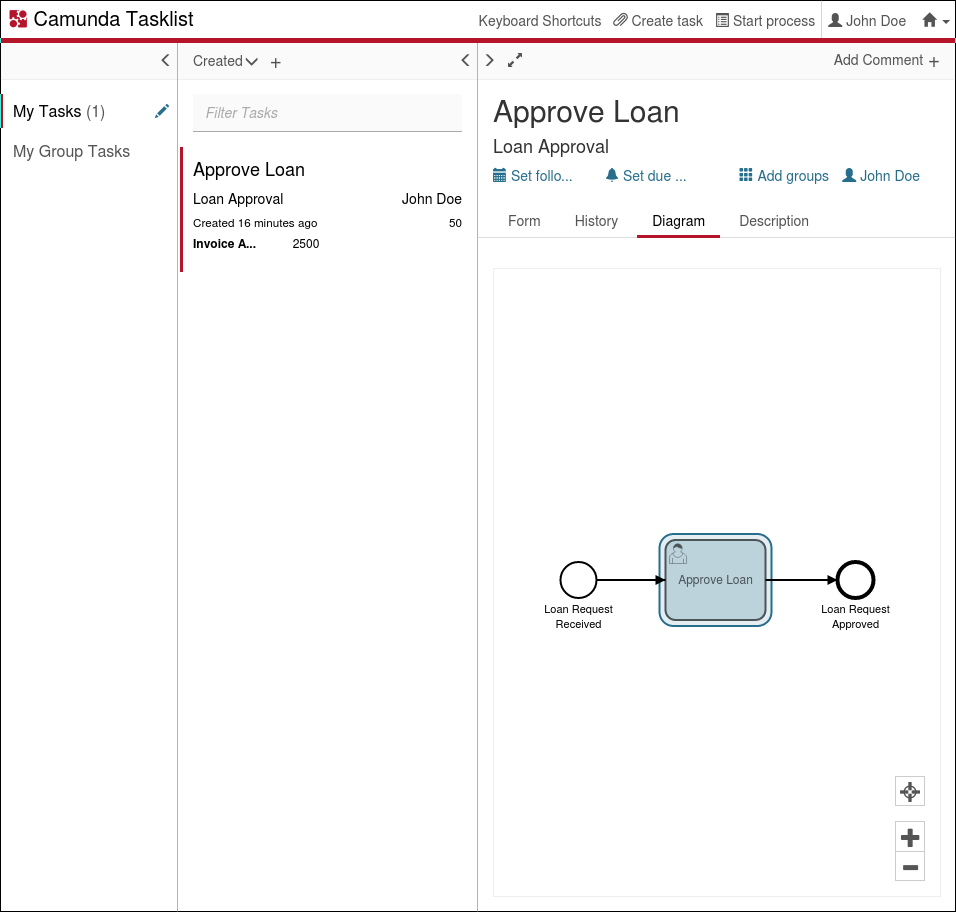
\includegraphics[width=\textwidth]{diagram.png}
\end{center}

Para trabajar en el task, selecciona el tab "Form". De nuevo, no hay un formulario asociado con el proceso. Clicka en "Load Variables". Esto muestra las variables que tú pusiste en el primer paso.

\begin{center}
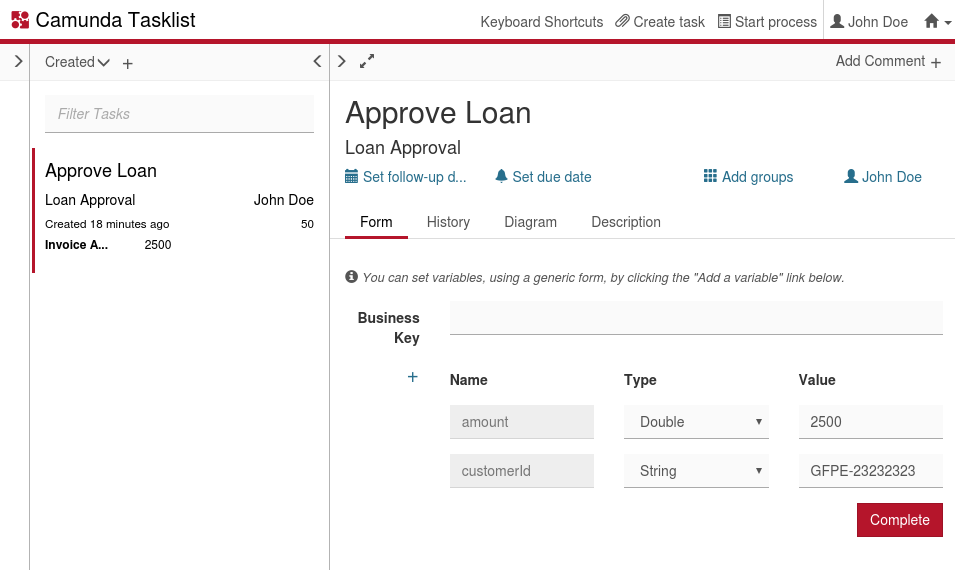
\includegraphics[width=\textwidth]{task-form-generic.png}
\end{center}

\newpage
\section{Agregar formulario HTML para Start y Task al proceso BPMN 2.0}

En el siguiente paso, queremos agregar un Task basado en un formulario en HTML a la aplicación.

\subsection{Agregar un formulario al Start}

Vuelve a Eclipse y agrega una carpeta llamada "forms" en la ruta "src/main/webapp/forms". Dentro de esta carpeta, agrega un archivo llamado "request-loan.html" y agrega el siguiente contenido en el archivo:

\begin{minted}[bgcolor=bg]{html}
<form name="requestLoan">
  <div class="form-group">
    <label for="customerId">Customer ID</label>
    <input class="form-control"
           cam-variable-type="String"
           cam-variable-name="customerId"
           name="customerId" />
  </div>
  <div class="form-group">
    <label for="amount">Amount</label>
    <input class="form-control"
           cam-variable-type="Double"
           cam-variable-name="amount"
           name="amount" />
  </div>
</form>
\end{minted}

Abre el diagrama con el Modeler. Clicka en el Start event. En la vista de propiedades, clicka en el tab "Forms" e inserta "embedded:app:forms/request-loan.html" en el campo "Form Key". Esto significa que queremos usar un formulario incrustado dentro del Tasklist y ese formulario se carga desde la aplicación.
Guarda tus cambios en el diagrama y actualiza Eclipse.

\begin{center}
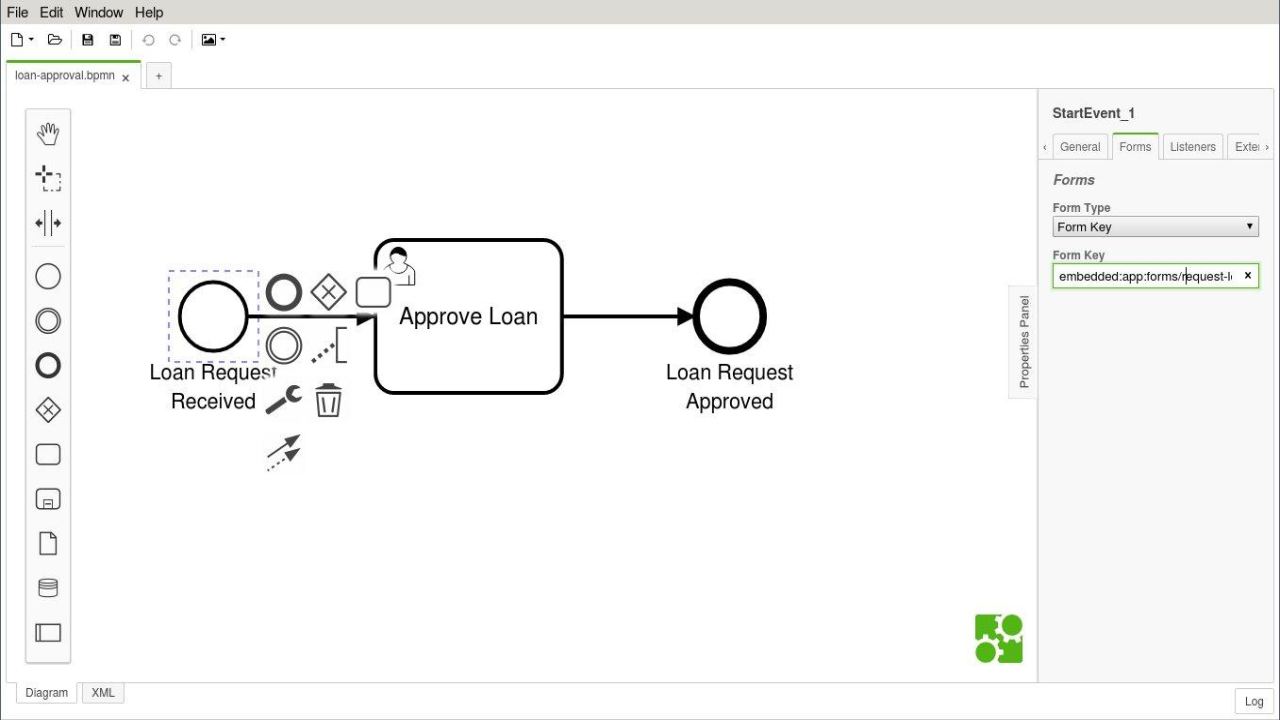
\includegraphics[width=\textwidth]{modeler-start-form.png}
\end{center}

\subsection{Agrega un formulario al Task}

El formulario para el Task, puede ser agregado del mismo modo. Agrega un archivo de nombre "approve-loan.html" en la ruta "src/main/webapp/forms" y agrega el siguiente contenido:

\begin{minted}[bgcolor=bg]{html}
<form name="approveLoan">
  <div class="form-group">
    <label for="customerId">Customer ID</label>
    <input class="form-control"
           cam-variable-type="String"
           cam-variable-name="customerId"
           name="customerId"
           readonly="true" />
  </div>
  <div class="form-group">
    <label for="amount">Amount</label>
    <input class="form-control"
           cam-variable-type="Double"
           cam-variable-name="amount"
           name ="amount" />
  </div>
</form>
\end{minted}

Luego de eso, abre el diagrama con el Modeler nuevamente. Clicka en el User Task. En la vista de propiedades, clicka en el tab "Forms" y agrega "embedded:app:forms/approve-loan.html" en el atributo "Form Key".

\subsection{Re-compila y despliega}

Cuando estés listo, guarda todos tus cambios, vuelve a compilar con el archivo "pom.xml" (del mismo modo que lo hicimos antes) y mueve el archivo "war" a la carpeta "webapps" (debes reemplazar el anterior).
Ahora, anda al Tasklist y empieza una nueva instancia del proceso "loan approval". Verás que se despliega el nuevo formulario.

\begin{center}
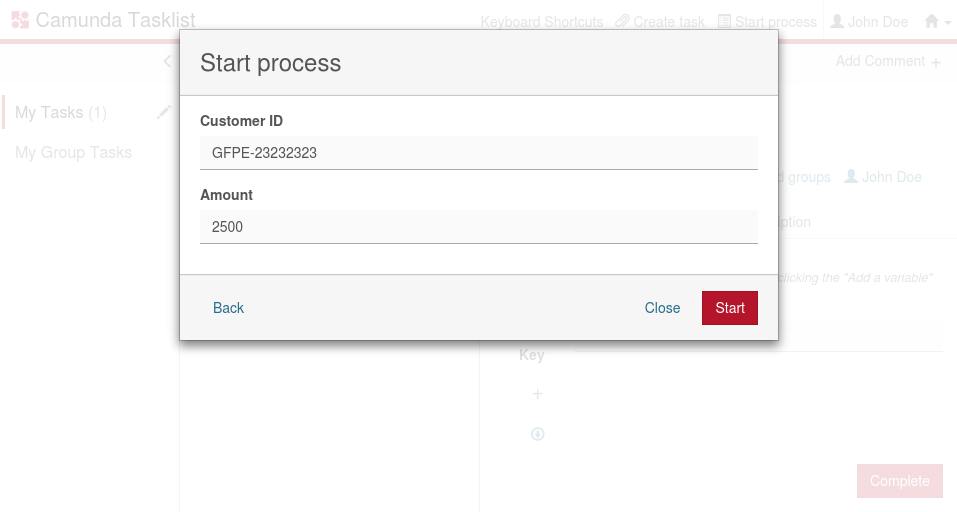
\includegraphics[width=\textwidth]{start-form-embedded.png}
\end{center}

Luego de empezar la nueca instacia del proceso, un task "Approve Loan" es asignado a john. Para trabajar en el task, inicia seisón como "john", selecciona el task en la lista de tasks y verás que el formulario personalizado es desplegado.

\begin{center}
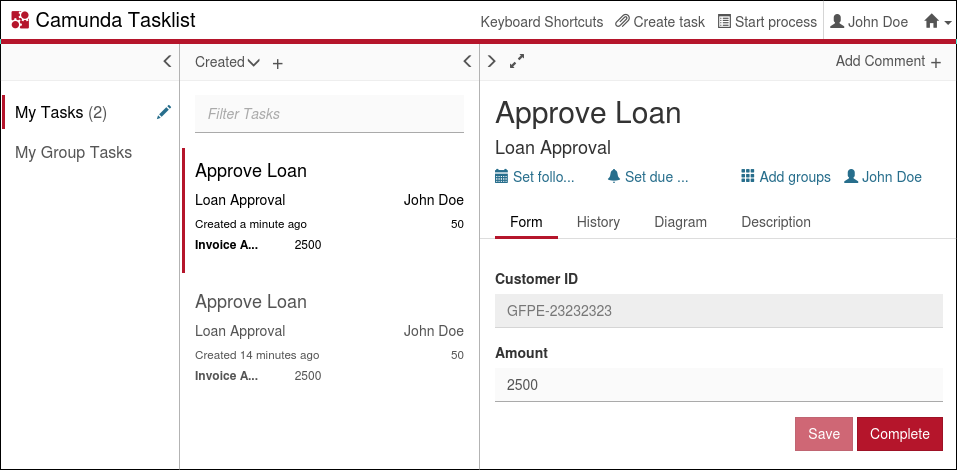
\includegraphics[width=\textwidth]{task-form-embedded.png}
\end{center}



\end{document}